\documentclass{article}
\usepackage[left=1.5cm, right=1.5cm, top=1.5cm, bottom=2cm]{geometry}
\usepackage[utf8]{inputenc}
\usepackage{amsmath,amsthm,stmaryrd,amssymb,bbm,amsfonts,amstext,graphicx,multicol,array}
\usepackage{subfigure}
\usepackage{xcolor}
\usepackage{enumitem}
\usepackage{indentfirst}
\usepackage{caption}
\usepackage{pdfpages}
\usepackage[numbers]{natbib} % Use natbib with numerical citations
\usepackage{hyperref}
\usepackage{float}
\usepackage{booktabs}
\usepackage{graphics, graphicx}
\usepackage{booktabs}
\usepackage{adjustbox}

\hypersetup{
    colorlinks=true,
    linkcolor=blue,
    urlcolor=blue,
    citecolor=blue
}

\setlength{\parindent}{2em}
\setlength{\parskip}{1em}
\renewcommand{\baselinestretch}{1.5}

\title{ECON2390 Fall 2024\\Applied Econometrics\\Problem Set 2}
\author{Adrien Foutelet}
\date{October 2024}

\begin{document}

\maketitle

\section{Regression Discontinuity Design}

%%%%%%%%%%%%%%%%%%%%%%%%%%%%%%%%%%%%%%%%%%%%%%%%%%%%%%%%%%%%%%%
\subsection{}

We run OLS to estimate the following model:
\[Y_m = \beta_0 + \beta_1 \text{PANwin}_m + \epsilon_m\]

We get the following estimates (see table \ref{tab:model1}).

\begin{table}[htbp]\centering
\def\sym#1{\ifmmode^{#1}\else\(^{#1}\)\fi}
\caption{Simple OLS regression model\label{tab:model1}}
\begin{tabular}{l*{1}{c}}
\toprule
                    &\multicolumn{1}{c}{Y}\\
\midrule
(mean) PANwin       &       0.904         \\
                    &      (0.06)         \\
\addlinespace
Constant            &       43.63\sym{***}\\
                    &      (4.58)         \\
\midrule
Observations        &         152         \\
\bottomrule
\multicolumn{2}{l}{\footnotesize \textit{t} statistics in parentheses}\\
\multicolumn{2}{l}{\footnotesize \sym{*} \(p<0.05\), \sym{**} \(p<0.01\), \sym{***} \(p<0.001\)}\\
\end{tabular}
\end{table}


The positive correlation between variables Y and PANwin that the coefficient suggests does not appear to be significant.

We may be facing endogeneity: it is where the homicide rate is high and the drug ttafficking organisations have strong presence that the party promoting radical anti drug policies is elected (reverse causality); PAN may have prioritized campaigning in dangerous areas where their agenda gave them the best chances to wind (selection); where the local culture is more martial, making PAN most popular, results from weaker state capacity which is suitable for criminal organisations to thrive (omitted variable bias). We need to isolate exogenous variations in PANwin to infer causal results.

For these reasons, \(\beta_1\) should be positively biased and \(\beta_0\) should be negatively biased.

%%%%%%%%%%%%%%%%%%%%%%%%%%%%%%%%%%%%%%%%%%%%%%%%%%%%%%%%%%%%%%%
\subsection{}

The key assumptions necessary for the fuzzy regression discontinuity design to be valid in Dell's analysis are:
\begin{itemize}
    \item Local monotonicity.\\
    There exists a neighborhood \(G\) around \(X=c\) where any individual in the population has one of the following treatment selection respondes:
    \begin{itemize}
        \item \(T=t_c \implies D_i(x)=1_{\{x\geq c\}} \)
        \item \(T=t_{at} \implies D_i(x)=1\)
        \item \(T=t_{at} \implies D_i(x)=0\).
    \end{itemize}
    \item Continuity:\\
    \(\forall t \in \{t_c,t_{at},t_{nt}\}, E(Y(1)\mid T=t,X=x), E(Y(0)\mid T=t,X=x), Pr(T=t \mid X=x) \text{ are continuous at } x=c\).
    \item First stage\\
    \( \lim_{x \to c^{-}}
    Pr(D=1 \mid X=x)
    \neq
    \lim_{x \to c^{+}}
    Pr(D=1 \mid X=x) \)
\end{itemize}

From the text (need to reconceile that):
\begin{itemize}   
    \item All relevant factors besides treatment vary smoothly at the threshold between a PAN victory and loss.
    \item Absence of selective sorting around the PAN win-loss threshold.
\end{itemize}

%%%%%%%%%%%%%%%%%%%%%%%%%%%%%%%%%%%%%%%%%%%%%%%%%%%%%%%%%%%%%%%

\subsection{}

Investigating whether the regression discontinuity design shows evidence of manipulation, we do a McCrary test for the following null hypothesis:

\[H_0: \text{ "The density of the running variable is continuous at the cutoff"}\]

We get the following results (see table \ref{tab:McCrary}):
\begin{table}[htbp]\centering
\caption{McCrary density test\label{tab:McCrary}}
\begin{tabular}{l*{1}{c}}
\hline\hline
            &\multicolumn{1}{c}{margin\_victory}\\
\hline
\hline
LogDensityRatio&     -0.0763\\
StdError    &       24.19\\
PValue      &       0.939\\
Bandwidth\_left&      0.0135\\
Bandwidth\_right&      0.0157\\
\hline\hline
\end{tabular}
\end{table}


Our high p-value implies that we fail to reject the null hypothesis, meaning that we find no evidene of significant difference in the density of the running variable on either side of the cutoff.

We get the following plot of the estimated density of the running variable on both sides of the cutoff (see figure \ref{fig:McCrary}). No visual discontinuity can be found in the density at the cutoff: the density is smooth. 

\begin{figure}[H]
    \centering
    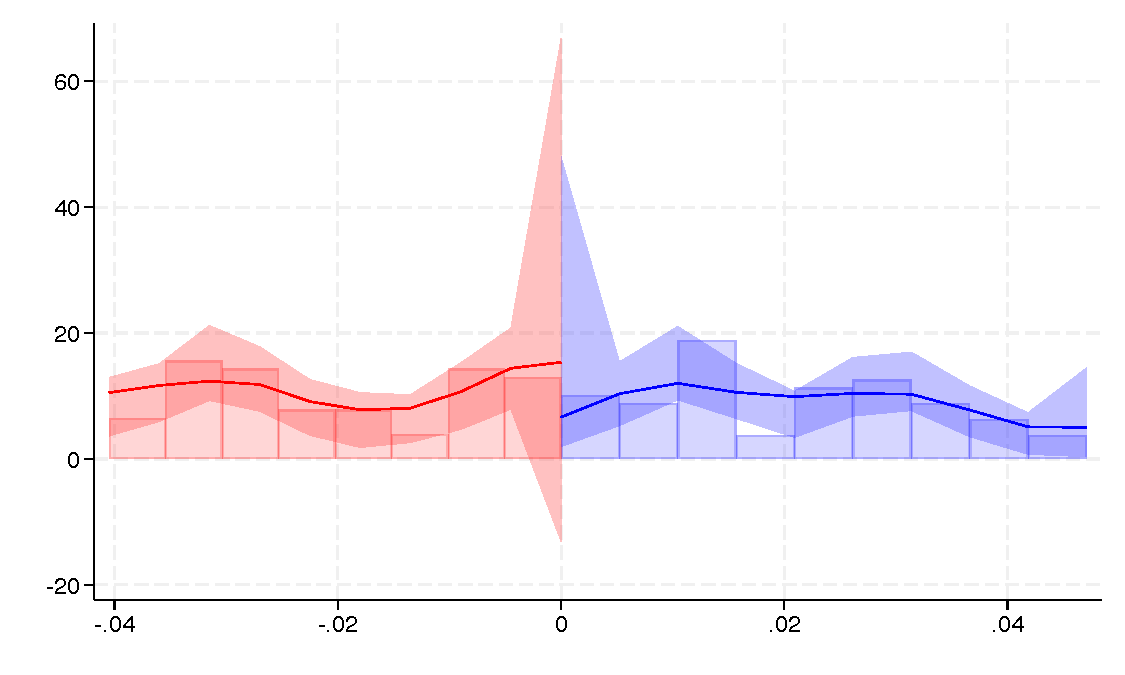
\includegraphics[width=\textwidth]{../outputs/mccrary_plot.pdf}
    \caption{McCrary test result plot}
    \label{fig:McCrary}
\end{figure}

All in all, the is no evidence of manipulation or sorting of the running variable at the cutoff.  This supports the validity of the RDD design.

%%%%%%%%%%%%%%%%%%%%%%%%%%%%%%%%%%%%%%%%%%%%%%%%%%%%%%%%%%%%%%%

\subsection{}

\begin{figure}[H]
    \centering
    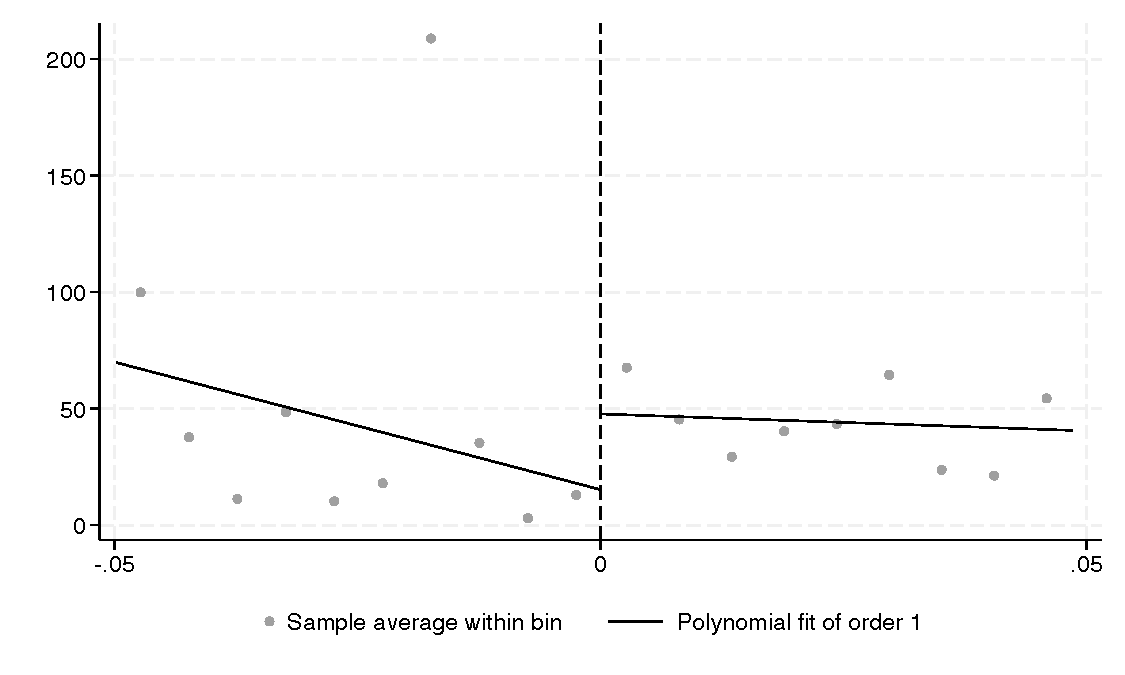
\includegraphics[scale=0.5]{../outputs/binned_scatter_esmv_linear_plot.pdf}
    \caption{Binned scatter plot of PAN victory margin and homicide rate (number of bins selected via mimicking variance evenly-spaced method using spacings estimators, linear specification)}
    \label{fig:binned_scatter_esmv_linear}
\end{figure}

\begin{figure}[H]
    \centering
    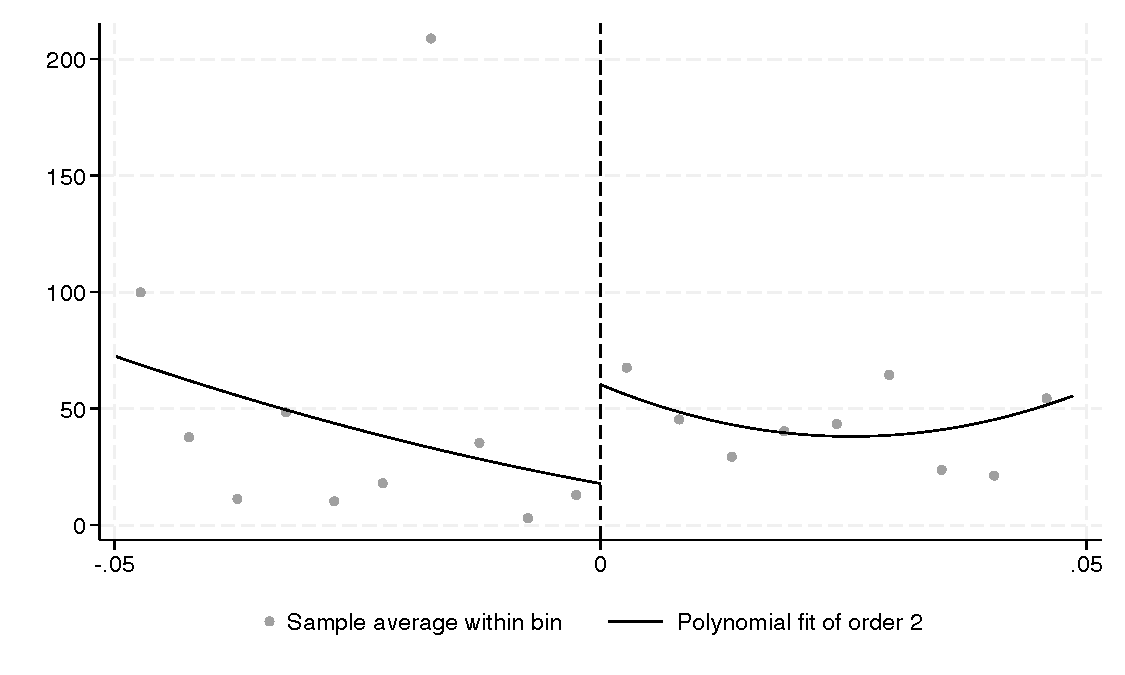
\includegraphics[scale=0.5]{../outputs/binned_scatter_esmv_quadratic_plot.pdf}
    \caption{Binned scatter plot of PAN victory margin and homicide rate (number of bins selected via mimicking variance evenly-spaced method using spacings estimators, quadratic specification)}
    \label{fig:binned_scatter_esmv_quadratic}
\end{figure}

\begin{figure}[H]
    \centering
    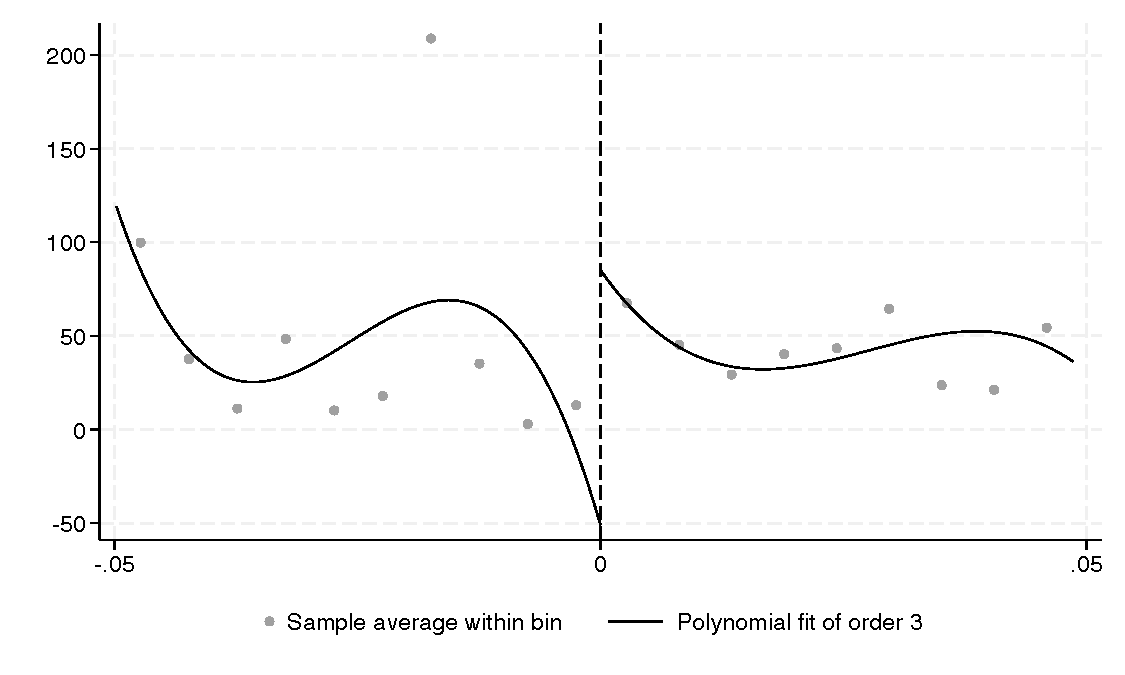
\includegraphics[scale=0.5]{../outputs/binned_scatter_esmv_cubic_plot.pdf}
    \caption{Binned scatter plot of PAN victory margin and homicide rate (number of bins selected via mimicking variance evenly-spaced method using spacings estimators, cubic specification)}
    \label{fig:binned_scatter_esmv_cubic}
\end{figure}

\begin{figure}[H]
    \centering
    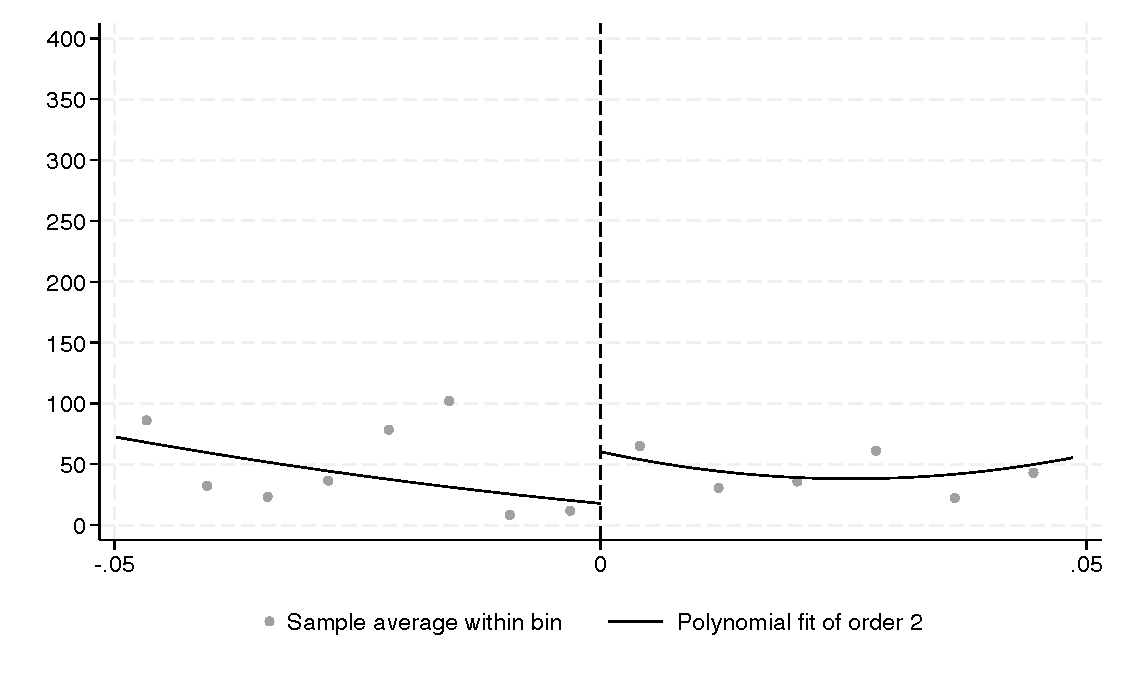
\includegraphics[scale=0.5]{../outputs/binned_scatter_es_cubic_plot.pdf}
    \caption{Binned scatter plot of PAN victory margin and homicide rate (number of bins selected via IMSE-optimal evenly-spaced method using spacings estimators, cubic specification)}
    \label{fig:binned_scatter_es_cubic}
\end{figure}

\begin{figure}[H]
    \centering
    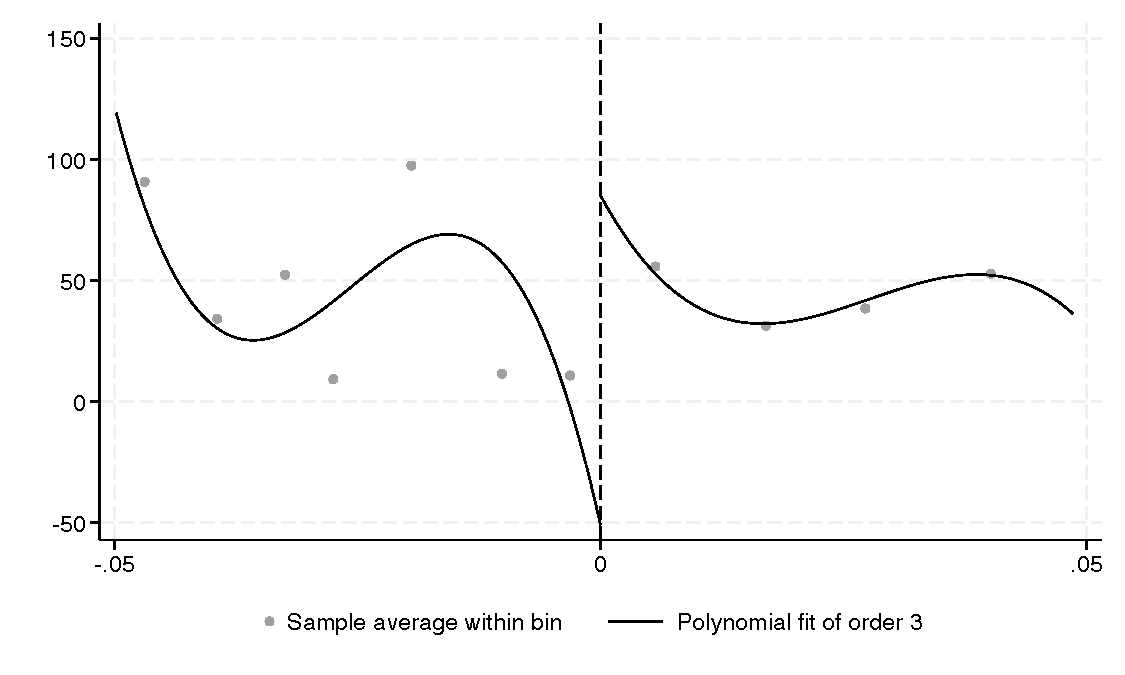
\includegraphics[scale=0.5]{../outputs/binned_scatter_qs_cubic_plot.pdf}
    \caption{Binned scatter plot of PAN victory margin and homicide rate (number of bins selected via IMSE-optimal quantile-spaced method using spacings estimators, cubic specification)}
    \label{fig:binned_scatter_qs_cubic}
\end{figure}

\begin{figure}[H]
    \centering
    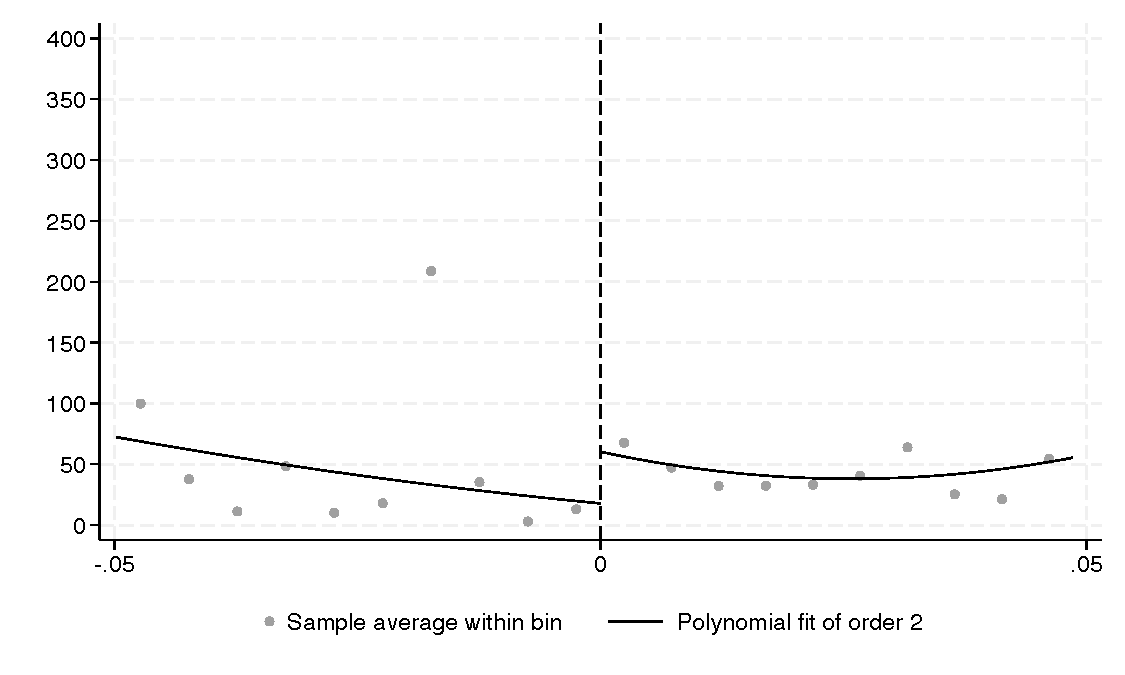
\includegraphics[scale=0.5]{../outputs/binned_scatter_10bins_cubic_plot.pdf}
    \caption{Binned scatter plot of PAN victory margin and homicide rate (number of bins bormatively set at 10, cubic specification)}
    \label{fig:binned_scatter_10bins_cubic}
\end{figure}

\begin{figure}[H]
    \centering
    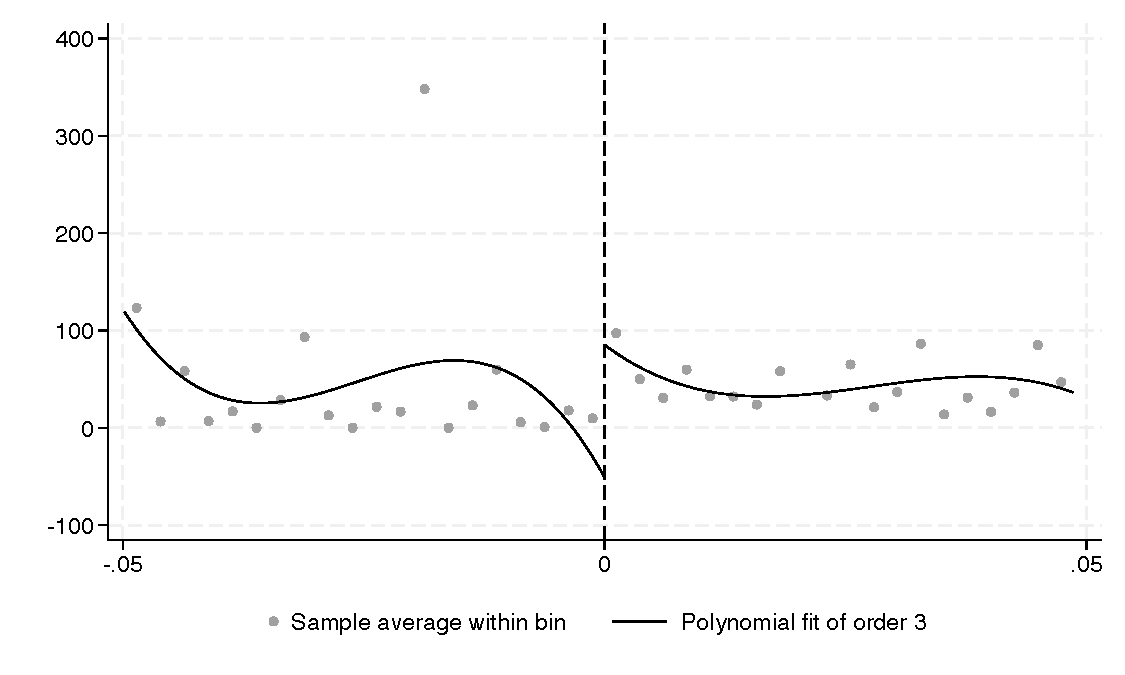
\includegraphics[scale=0.5]{../outputs/binned_scatter_20bins_cubic_plot.pdf}
    \caption{Binned scatter plot of PAN victory margin and homicide rate (number of bins bormatively set at 20, cubic specification)}
    \label{fig:binned_scatter_20bins_cubic}
\end{figure}

The discontinuity at the cutoff is robust to the three polynomial specifications.

The smaller the number of bins, the larger the discontinuity.

%%%%%%%%%%%%%%%%%%%%%%%%%%%%%%%%%%%%%%%%%%%%%%%%%%%%%%%%%%%%%%%

\subsection{}

We get the following estimates (see table \ref{tab:model2}).

\begin{table}[htbp]\centering
\def\sym#1{\ifmmode^{#1}\else\(^{#1}\)\fi}
\caption{Non-parametric and parametric RDD models\label{tab:model2}}
\begin{tabular}{l*{4}{c}}
\toprule
                    &\multicolumn{1}{c}{Non-para tri lin}&\multicolumn{1}{c}{Non-para tri quad}&\multicolumn{1}{c}{Para lin}&\multicolumn{1}{c}{Para quad}\\
\midrule
RD\_Estimate         &       80.25\sym{*}  &       93.93         &                     &                     \\
                    &      (2.25)         &      (1.92)         &                     &                     \\
\addlinespace
(mean) spread       &                     &                     &       979.5         &      2697.6         \\
                    &                     &                     &      (0.36)         &      (0.39)         \\
\addlinespace
(mean) PANwin       &                     &                     &       69.99\sym{**} &       81.79\sym{*}  \\
                    &                     &                     &      (2.91)         &      (2.57)         \\
\addlinespace
(mean) PANwin=1 $\times$ (mean) spread&                     &                     &     -5770.9         &    -12951.7         \\
                    &                     &                     &     (-1.50)         &     (-1.31)         \\
\addlinespace
(mean) spread squared&                     &                     &                     &    260133.0         \\
                    &                     &                     &                     &      (0.54)         \\
\addlinespace
(mean) PANwin=1 $\times$ (mean) spread squared&                     &                     &                     &    138247.6         \\
                    &                     &                     &                     &      (0.21)         \\
\addlinespace
Constant            &                     &                     &       12.95         &       14.37         \\
                    &                     &                     &      (0.78)         &      (0.66)         \\
\midrule
Observations        &         152         &         152         &          38         &          54         \\
\bottomrule
\multicolumn{5}{l}{\footnotesize \textit{t} statistics in parentheses}\\
\multicolumn{5}{l}{\footnotesize \sym{*} \(p<0.05\), \sym{**} \(p<0.01\), \sym{***} \(p<0.001\)}\\
\end{tabular}
\end{table}


%%%%%%%%%%%%%%%%%%%%%%%%%%%%%%%%%%%%%%%%%%%%%%%%%%%%%%%%%%%%%%%

\subsection{}

We get the following estimates (see table \ref{tab:model2-robustness}).

\begin{table}[htbp]\centering
\def\sym#1{\ifmmode^{#1}\else\(^{#1}\)\fi}
\caption{RDD model robustness\label{tab:model2-robustness}}
\begin{tabular}{l*{4}{c}}
\toprule
                    &\multicolumn{1}{c}{Para tri lin}&\multicolumn{1}{c}{Para tri lin 5\%}&\multicolumn{1}{c}{Para tri lin 10\%}&\multicolumn{1}{c}{Para tri lin 20\%}\\
\midrule
RD\_Estimate         &       80.25\sym{*}  &       80.25\sym{*}  &       98.36\sym{*}  &       48.95         \\
                    &      (2.25)         &      (2.25)         &      (2.14)         &      (1.00)         \\
\midrule
Observations        &         152         &         152         &         151         &         144         \\
\bottomrule
\multicolumn{5}{l}{\footnotesize \textit{t} statistics in parentheses}\\
\multicolumn{5}{l}{\footnotesize \sym{*} \(p<0.05\), \sym{**} \(p<0.01\), \sym{***} \(p<0.001\)}\\
\end{tabular}
\end{table}


\begin{figure}[H]
    \centering
    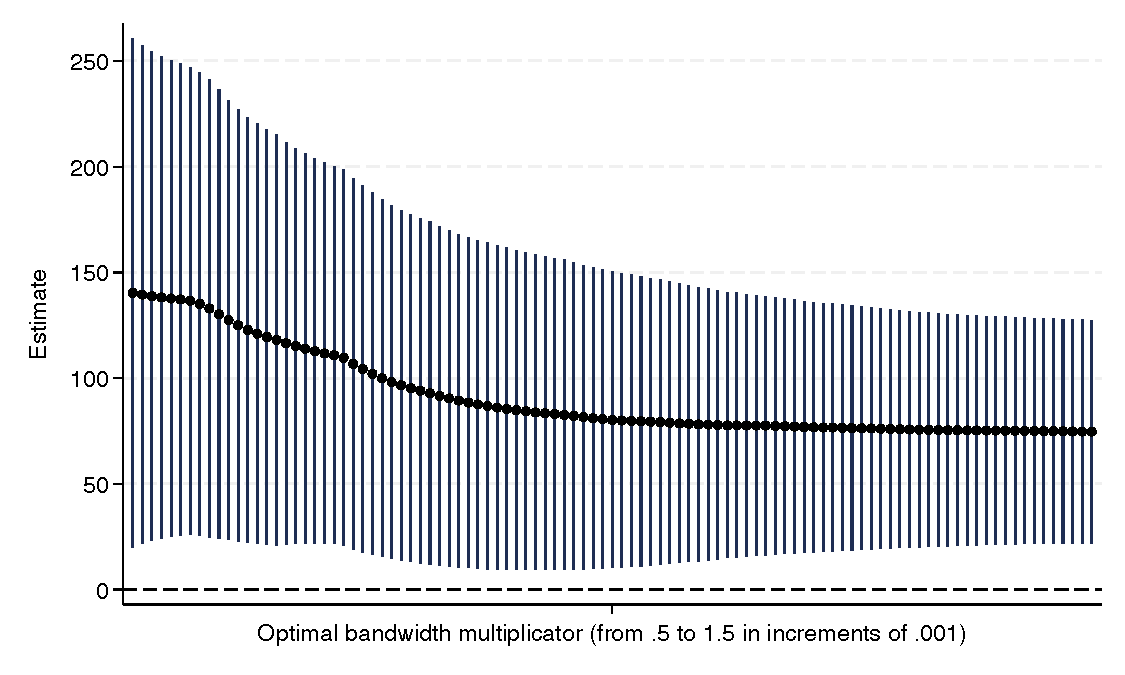
\includegraphics[scale=0.5]{../outputs/model2_robustness_plot.pdf}
    \caption{RDD model robustness}
    \label{fig:model2-robustness}
\end{figure}

%%%%%%%%%%%%%%%%%%%%%%%%%%%%%%%%%%%%%%%%%%%%%%%%%%%%%%%%%%%%%%%

\subsection{}

John Marshall's concern about compensating differentials in Politician Characteristic Regression Discontinuity (PCRD) designs revolves around the idea that these designs fail to isolate the pure effect of a politician's characteristic (e.g., gender, party affiliation) because other characteristics, known as compensating differentials, influence both the election outcome and downstream effects.

For example, if voters are biased against women, female candidates in close elections may need to compensate by having higher levels of competence or qualifications than their male opponents. The characteristic of interest (e.g., gender) correlates with compensating differentials that offset its impact (e.g., competence).

This means that PCRD designs compare candidates who are not equivalent on other key traits, leading to biased estimates of the effect of the characteristic of interest, since the effect measured is a compound treatment effect of the characteristic of interest and the compensation differentials.

Marshall recommends to attempt to measure compensating differentials to bound or reinterpret the results.

Dell leverages close elections to argue that PAN mayoral victories causally increase drug-related violence. The compensating differentials from winning PAN condidates may be their strong-willed disruptive and uncomproming characters (prone to get drug dealers' backs up), their expected lower level of corruption (prone to increase violence from the mobsters), their stronger connections with federal authorities (prone to make anti crime policies even stronger locally), or their lack of knowledge in sociology of deviance (prone to make them both attractively radical and acting without tact). There would then be selection of these traits for the mayors in the treatment group. 

\subsection{}

\begin{figure}
    \centering
    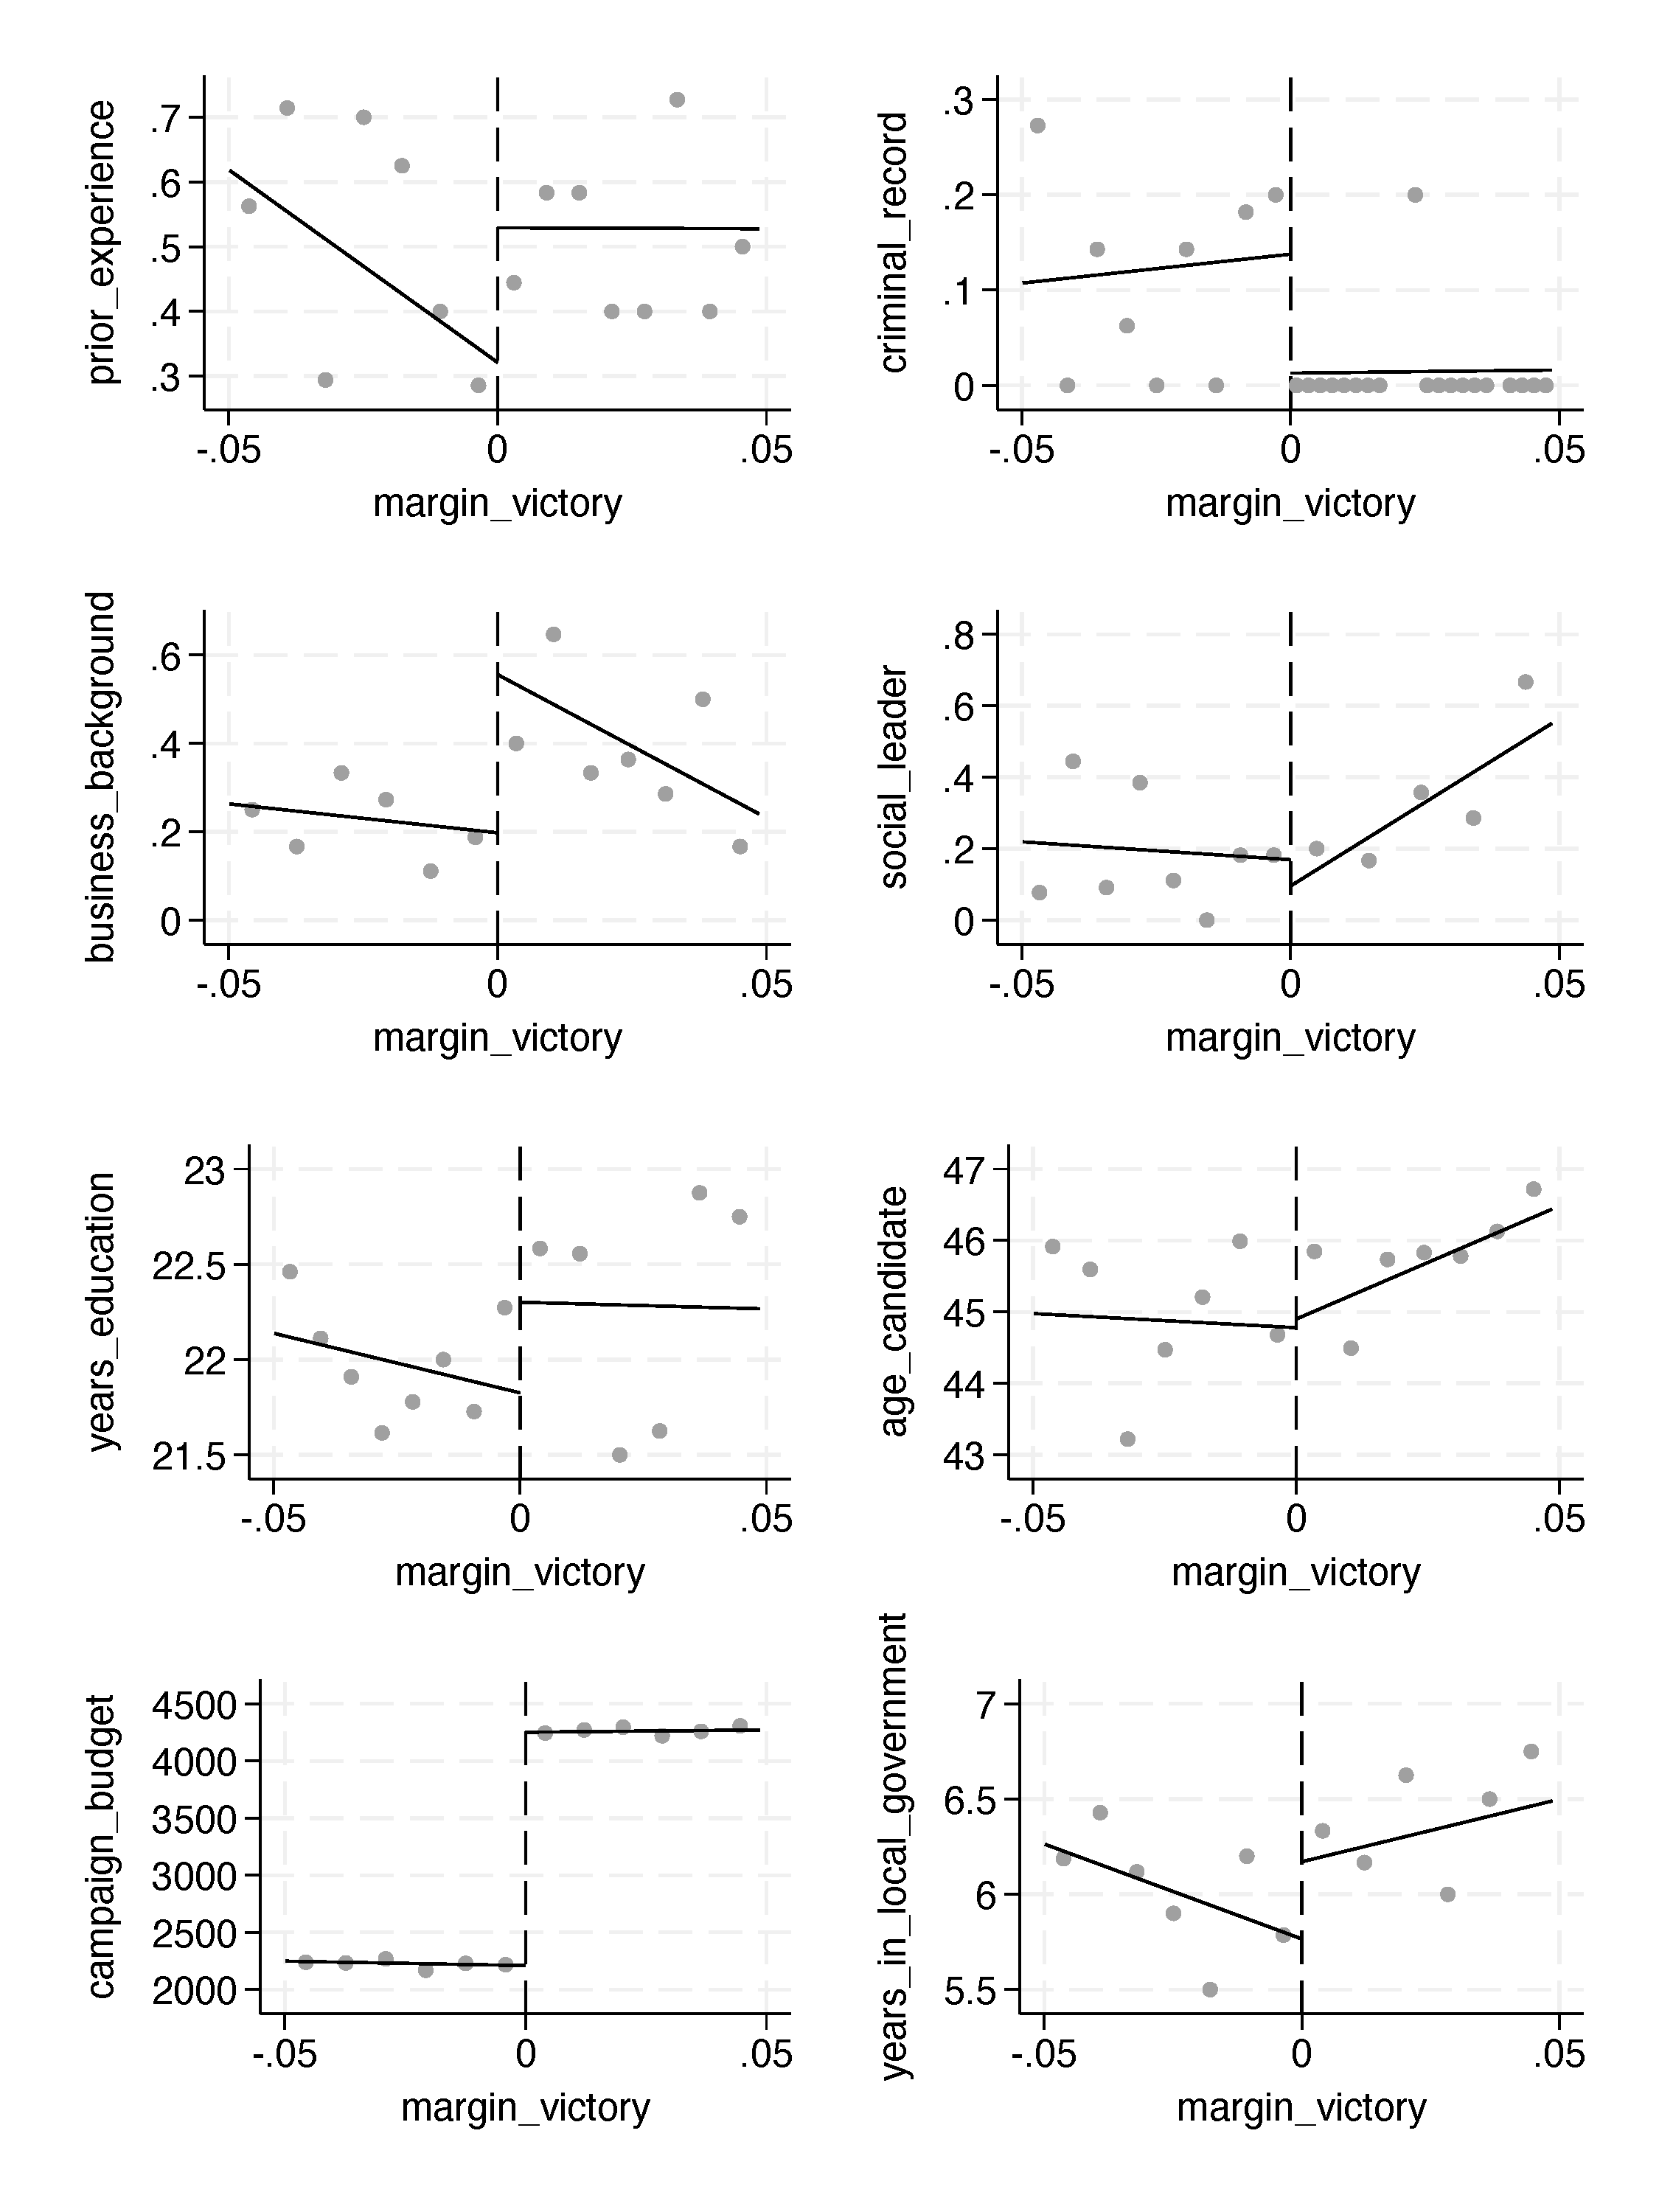
\includegraphics[scale=0.5]{../outputs/characteristics_binned_scatter_esmv_linear_plot.pdf}
    \caption{RDD model robustness}
    \label{fig:characteristics}
\end{figure}

\begin{figure}[H]
    \centering
    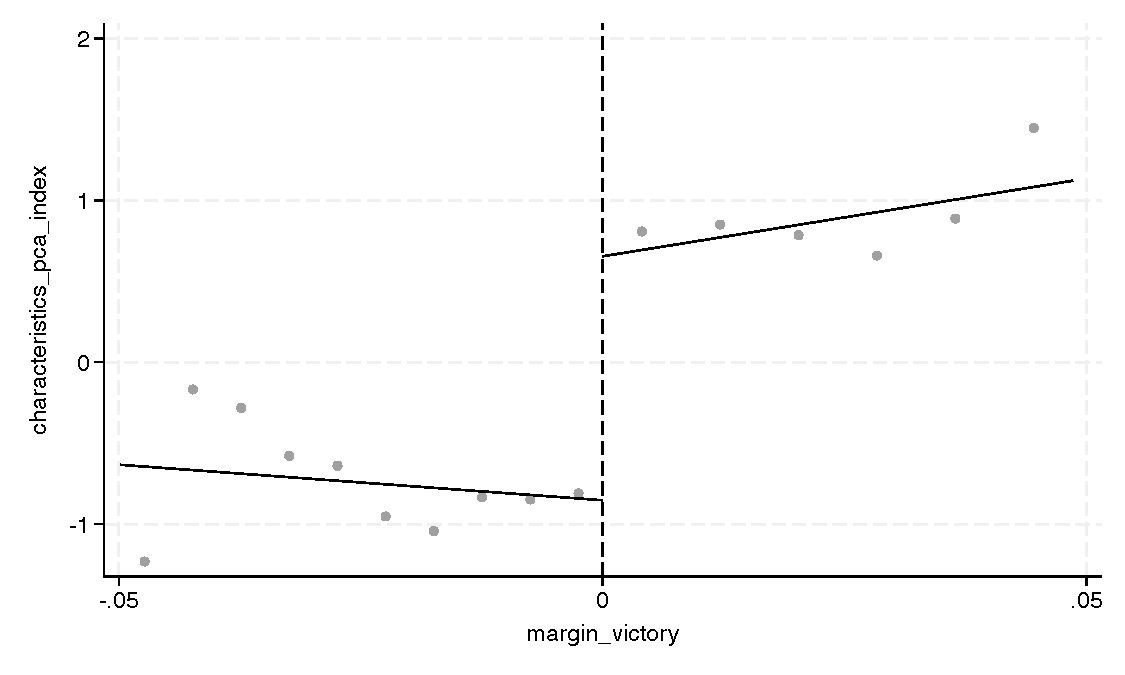
\includegraphics[scale=0.5]{../outputs/characteristics_pca_index_binned_scatter_esmv_linear_plot.pdf}
    \caption{RDD model robustness}
    \label{fig:pca_index}
\end{figure}

\def\sym#1{\ifmmode^{#1}\else\(^{#1}\)\fi}
\begin{adjustbox}{max
width={\textwidth},caption={Candidate characteristic RDD analysis\label{tab:characteristics}},nofloat=table}
\begin{tabular}{l*{9}{c}}
\toprule
                    &\multicolumn{1}{c}{pca\_index}&\multicolumn{1}{c}{prior\_experience}&\multicolumn{1}{c}{criminal\_record}&\multicolumn{1}{c}{business\_background}&\multicolumn{1}{c}{social\_leader}&\multicolumn{1}{c}{years\_education}&\multicolumn{1}{c}{age\_candidate}&\multicolumn{1}{c}{campaign\_budget}&\multicolumn{1}{c}{years\_in\_local\_government}\\
\midrule
RD\_Estimate         &       1.934\sym{**} &       0.179         &      -0.303         &      0.0150         &      0.0274         &       0.525         &       1.629         &      2038.0\sym{***}&       0.673         \\
                    &      (2.84)         &      (0.60)         &     (-1.26)         &      (0.05)         &      (0.11)         &      (0.60)         &      (0.98)         &     (21.42)         &      (0.93)         \\
\midrule
Observations        &         152         &         152         &         152         &         152         &         152         &         152         &         152         &         152         &         152         \\
\bottomrule
\multicolumn{10}{p{\textwidth}}{\centering \footnotesize \textit{t} statistics in parentheses}\\
\multicolumn{10}{p{\textwidth}}{\centering \footnotesize \sym{*} \(p<0.05\), \sym{**} \(p<0.01\), \sym{***} \(p<0.001\)}\\
\end{tabular}\end{adjustbox}


We get the following estimates (see table \ref{tab:characteristics}).

Covariate adjustment in a RDD is not sufficient to address the problem of compensating differentials, because these differentials introduce biases that are inherently linked to both observable and unobservable characteristics. Even if observable covariates balanced or controlled for, unobservable characteristics (e.g., competence) could vary discontinuously at the threshold, biasing the treatment effect. Also, covariates may include variables affected by the treatment itself (e.g., campaign funding postulated by voter - donors - and party organiztion expectations of winning). Including these covariates introduces post-treatment bias (conditioning on factors influenced by the treatmet), contaminating causal estimates.

All in all, covariate adjustment can reduce noise and account for observable imbalances, but it cannot fully address biases introduced by compensating differentials, especially when unobservable factors are at play.

%%%%%%%%%%%%%%%%%%%%%%%%%%%%%%%%%%%%%%%%%%%%%%%%%%%%%%%%%%%%%%%

\subsection{}

To bound the effect of a PAN mayor on the homicide rate, we implement:
\[
\hat{\tau}^{corr}_{PCRD}
=\hat{\tau}_{PCRD}
-\sum_{k} \hat{\gamma}_k \hat{\delta}_k
\]
With:
\begin{itemize}
    \item index \(i\) for candidates,
    \item index \(d\) for district,
    \item index \(k\) for covariates,
    \item \(\hat{\gamma}_k\) an estimate of the LATE of each compensating differential \(Z_{idk}\),
    \item
    \(
    \delta_k
    =
    E[Z_{idk}\mid \Delta_d = 0, X_{id}=1, X_{jd}=0]
    -
    E[Z_{idk}\mid \Delta_d = 0, X_{id}=0, X_{jd}=1]
    \),
    \item
    \(
    \Delta_d
    =
    V_{id}-V_{0d}
    \),
    \item \( V_{id}\) and \(V{0d}\) the vote shares of the most popular candidates of types \(X_{id}=1\) and \(X_{id}=1\) respectively,
    \item  \(X_{id}\) a binary characteristic that helps candidate \(i\) win votes.
\end{itemize}

\begin{figure}[H]
    \centering
    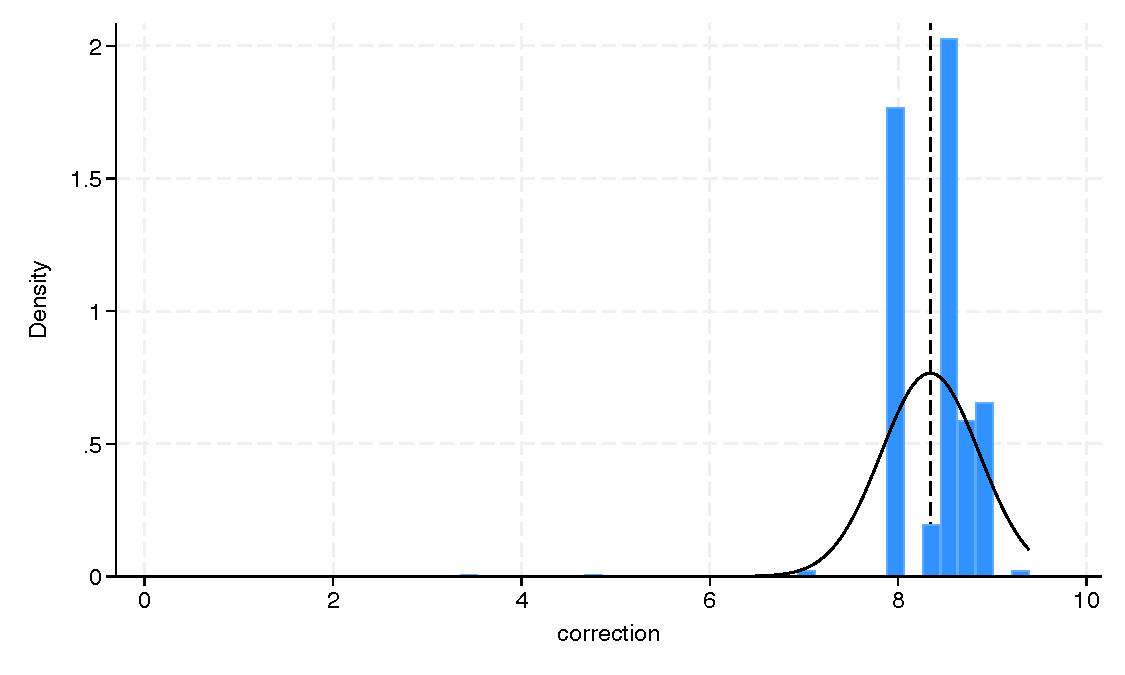
\includegraphics[scale=0.5]{../outputs/correction_term_distribution_plot.pdf}
    \caption{Distribution of the computed correction term}
    \label{fig:correction}
\end{figure}

Recalling that \(\hat{\tau}_{PCRD} = 80.25^{*}\text{ }(2.25)\), the sign and the significance level of our estimate are robust to the (observable) effect of compensating differentials.

\section{}

\subsection{}

\begin{table}[htbp]\centering
\def\sym#1{\ifmmode^{#1}\else\(^{#1}\)\fi}
\caption{IV\label{tab:IV-2SLS-IV-Wald}}
\begin{tabular}{l*{2}{c}}
\toprule
                    &\multicolumn{1}{c}{2SLS}&\multicolumn{1}{c}{Wald}\\
\midrule
D                   &       7.633\sym{***}&       7.633\sym{***}\\
                    &     (46.28)         &     (46.02)         \\
\addlinespace
x1                  &       0.124\sym{*}  &                     \\
                    &      (2.25)         &                     \\
\addlinespace
x2                  &      0.0708         &                     \\
                    &      (1.44)         &                     \\
\addlinespace
x1x2                &       0.282\sym{***}&                     \\
                    &      (3.84)         &                     \\
\addlinespace
Constant            &       1.039\sym{***}&       1.208\sym{***}\\
                    &     (10.49)         &     (13.17)         \\
\midrule
Observations        &       10000         &       10000         \\
\bottomrule
\multicolumn{3}{l}{\footnotesize \textit{t} statistics in parentheses}\\
\multicolumn{3}{l}{\footnotesize \sym{*} \(p<0.05\), \sym{**} \(p<0.01\), \sym{***} \(p<0.001\)}\\
\end{tabular}
\end{table}


The 2SLS and residualzed Wald estimators are equal.

\subsection{}

A researcher observing \((Y_i,D_i,Z_i,X_i)\) would identify the conditional-on-\(X_i\) LATESs \(E[Y_i(1)-Y_i(0) \mid X_i, G = CP]\) by 2SLS on observations such that \((X_i = Z_i)\). This is equivalent to eestimating the structural model by OLS on this restricted dataset.

\def\sym#1{\ifmmode^{#1}\else\(^{#1}\)\fi}
\begin{adjustbox}{max
width={\textwidth},caption={Unconditional and conditional LATEs \label{tab:IV-2SLS-IV-Wald-CP}},nofloat=table}
\begin{tabular}{l*{8}{c}}
\toprule
                    &\multicolumn{1}{c}{2SLS X=(0,0)}&\multicolumn{1}{c}{LATE X=(0,0)}&\multicolumn{1}{c}{2SLS X=(1,0)}&\multicolumn{1}{c}{LATE X=(1,0)}&\multicolumn{1}{c}{2SLS X=(0,1)}&\multicolumn{1}{c}{LATE X=(0,1)}&\multicolumn{1}{c}{2SLS X=(1,1)}&\multicolumn{1}{c}{LATE X=(1,1)}\\
\midrule
D                   &       6.680\sym{***}&       5.911\sym{***}&       8.434\sym{***}&       8.126\sym{***}&       6.502\sym{***}&       7.086\sym{***}&       9.139\sym{***}&       9.062\sym{***}\\
                    &     (16.95)         &     (60.13)         &     (37.83)         &     (93.68)         &     (12.48)         &     (73.80)         &     (47.82)         &    (103.33)         \\
\addlinespace
Constant            &       1.587\sym{***}&      0.0624         &       0.828\sym{***}&     -0.0380         &       1.808\sym{***}&     -0.0179         &       0.600\sym{***}&     -0.0129         \\
                    &      (6.97)         &      (0.99)         &      (8.78)         &     (-1.00)         &      (5.70)         &     (-0.24)         &      (5.08)         &     (-0.16)         \\
\midrule
Observations        &        2500         &         417         &        2500         &         833         &        2500         &         417         &        2500         &         833         \\
\bottomrule
\multicolumn{9}{p{\textwidth}}{\centering \footnotesize \textit{t} statistics in parentheses}\\
\multicolumn{9}{p{\textwidth}}{\centering \footnotesize \sym{*} \(p<0.05\), \sym{**} \(p<0.01\), \sym{***} \(p<0.001\)}\\
\end{tabular}\end{adjustbox}


\subsection{}

\begin{table}[htbp]\centering
\caption{Weights and convex weighted average of the conditional LATEs\label{tab:Angrist}}
\begin{tabular}{l*{1}{c}}
\hline\hline
            &\multicolumn{1}{c}{}\\
\hline
Beta 2SLS   &       7.633\\
\hline
Weight00    &       0.546\\
Weight10    &       1.516\\
Weight01    &       0.569\\
Weight11    &       1.369\\
LATEsCvxWghtedAvg&       7.877\\
\hline\hline
\end{tabular}
\end{table}



We get \(\hat{Beta}_{2SLS} =7.8765399\), which is close to our initial 2SLS estimation.

The group that gets more weight is \(X=(1,0)\).


\begin{thebibliography}{9}

\bibitem{dell2015}
Dell, Melissa. “Trafficking Networks and the Mexican Drug War.” American Economic Review 105, no. 6 (2015): 1738-1779.

\bibitem{marshall2024}
Marshall, J. (2024), Can Close Election Regression Discontinuity Designs Identify Effects of Winning Politician Characteristics?. American Journal of Political Science, 68: 494-510.

\end{thebibliography}

\end{document}